\documentclass[10pt]{article}
\usepackage[letterpaper, margin=1in]{geometry}
\usepackage[pdftex]{graphicx}
\usepackage[utf8]{inputenc}
\usepackage{tikz, wrapfig, amssymb, array, mathtools, circuitikz, physics, parskip, hyperref}
\usepackage{enumitem}
\usepackage{tkz-euclide}
\usepackage{titlesec}
\usepackage{lipsum}
\usepackage[english]{babel}
\usepackage{amsmath, amsthm}
\usepackage{fancyhdr}
\usepackage{xcoffins}
\usepackage{tcolorbox}
\usepackage{../local}


\newcommand{\classcode}{Physics 5CL}
\newcommand{\classname}{Introduction to Experimental Physics II}
\renewcommand{\maketitle}{%
\hrule height4pt
\large{Eric Du \hfill \classcode}
\newline
\large{Prelab 04} \large{\hfill \classname \hfill} \large{\today}
\hrule height4pt \vskip .7em
\normalsize
}
\linespread{1.1}
\begin{document}
    \maketitle
    \section*{Problem 1}

    Light of known wavelength $\lambda_{known}$ is incident on a diffraction grating and forms a pattern on a screen a distance $L$ away. The first maximum occurs at position $y_{known}$ relative to the central maximum. When light of unknown wavelength $\lambda_{un}$ is incident on the grating, the first maximmum occurs at position $y_{un}$

    \begin{enumerate}[label=\alph*)]
        \item Determine $\lambda_{un}$ in terms of $\lambda_{knonw}, y_{known}$ and $y_{un}$
        

        \begin{solution}
            We have the relation that 

            \[ \sin \theta = \pm \frac{m\lambda}{D}\]

            So using the small angle approximation, $\sin \theta \approx \tan \theta = \frac{y}{L}$, so therefore we have: 

            \[ \frac{y_{known}}{L} = \frac{\lambda_{known}}{D} \implies D = \frac{\lambda_{known}L}{y_{known}}\]

            Similarly with the light of wavelength $\lambda_{un}$, 

            \[ D = \frac{\lambda_{un}L}{y_{un}}\] 

            So therefore, we can equate the two equations, since we're using the same diffraction grating, which gives us 

            \[ \lambda_{un} = \frac{y_{un}\lambda_{known}}{y_{known}}\]
        \end{solution}
    \end{enumerate}

    \pagebreak
    \section*{Problem 2}

        Consider the photoelectric effect simulation made by PhET Interactive Simulations group at University of Colorado, Boulder, available for download at \url{https://phet.colorado.edu/en/simulation/photoelectric}

        Set the intensity to 100\%, the battery voltage to 0.0V, and the material to sodium (Na). 

        \begin{enumerate}[start, label=\alph*)]
            \item Determine the threshold wavelength, threshold frequency, and work function of incident light 
            \begin{solution}
                I ran the simulation, and found that the minimum wavelength occurs at $\lambda_{min} = 539$ nm, which corresponds to a wavelength of $5.56 \times 10^{14}$ Hz using $f = \frac{c}{\lambda}$. Therefore, the work function is given by 

                \[ hf_0 = 3.68\times 10^{-19} \text{ Js}\]

                which also corresponds to 2.3 eV.
            \end{solution}

            \item Set the wavelength to 300 nm and take some data to show that the photocurrent is directly proportional to intensity.
            
            \begin{solution}
                Refer to the following chart: 

                \begin{center}
                    \begin{tabular}{l|l}
                        Intensity & Photocurrent \\ \hline
                        100\%     & 0.556        \\
                        80\%      & 0.445        \\
                        60\%      & 0.333        \\
                        40\%      & 0.222        \\
                        20\%      & 0.111        \\
                        0\%       & 0           
                    \end{tabular}
                \end{center}

                I plotted this in python:

                \begin{center}
                    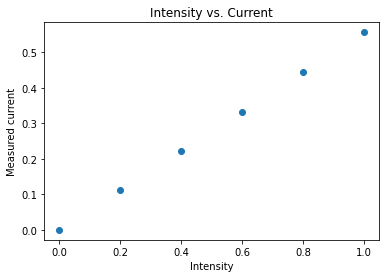
\includegraphics[scale=0.8]{intensityvscurrent.png}
                \end{center}

                And just to confirm it's linear, I performed a linear fit: 

                \begin{center}
                    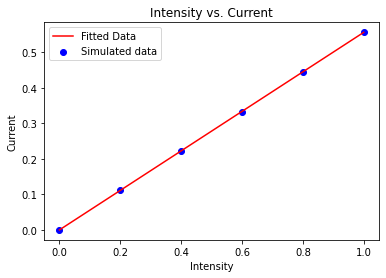
\includegraphics[scale=0.8]{intensityvscurrentwfit.png}
                \end{center}

                Python also tells me that the constant of proportionality is 0.555, but I'm not entirely sure how to confirm whether it makes sense.
            \end{solution}

            \item Experiemntally find the (simulated) stopping voltages for wavelengths of 300 nm and 200 nm and use this to measure $h$. 
            
            \begin{solution}
                The simulated stopping voltages for 300 nm and 200 nm are -1.79V and -3.87V respectively. To measure $h$, we use:

                \[ eV_{stop} = h(f - f_0) \implies h = \frac{eV_{stop}}{f - f_0}\]

                the frequency of 300 nm light is $9.99 \times 10^{14}$ Hz, so this gives us 

                \[ h = 6.46 \times 10^{-34}\]

                which is relatively close to the actual value of Planck's constant. Doing the same for 200nm light gives 

                \[ h = 6.55\times 10^{-34}\]
            \end{solution}
        \end{enumerate}

        With the wavelength set to 200 nm, adjust the battery to the stopping voltage. Then adjust the wavelength to 300 nm (without adjusting the battery). The current should still be exactly zero. 

        \begin{enumerate}[resume, label=\alph*)]
            \item Explain why the voltage shown on the battery does \textit{not} represent the stopping voltage in this case. Why are we just reading zero current and not a negative current? Why is this observation important for when you get into the lab and need to take real data?
            
            \begin{solution}
                The voltage shown on the battery does not represent the stopping voltage becuase it's not the lowest voltage which gives us zero current. The reason we don't measure any current is because there aren't any electrons that reach the anode, and so no current is measured. The reason we don't measure negative current is because the photocathode and anode are placed far enough apart that they don't act as a capacitor (or a very weak one at that), so there is no potential difference, and thus no circuit is formed.

                This is important when taking real data because it means we need to make sure that we're measuring the actual stopping voltage and not a voltage greater than that, since observationally both voltages look identical.
            \end{solution}
        \end{enumerate}
\end{document}